\documentclass[a4paper,11pt,exos]{nsi} % COMPILE WITH DRAFT
\usepackage{pifont}
\usepackage{fontawesome5}
\geometry{margin=2cm}




\begin{document}
\classe{\premiere spé}
\titre{DL }
\maketitle

\subsection*{Contrôle qualité}
\dleft{12cm}{Une entreprise fabrique des tablettes de chocolat. Le service de contrôle
qualité effectue plusieurs types de contrôle.\\
L'un d'eux consiste à vérifier le taux d’humidité qui doit être de 7 \% pour que les fèves soient considérées comme conformes.}
{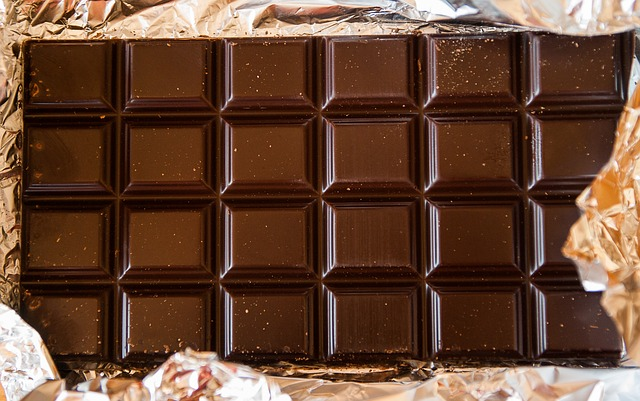
\includegraphics[width=4.5cm]{chocolate-1277002_640.jpg}}
L’entreprise a trois fournisseurs différents :
\begin{enumerate}[label=\textbullet]
    \item Le fournisseur 1 procure la moitié du stock de fèves, 98 \% de sa production respecte le taux d’humidité.
    \item Le fournisseur 2 fournit 30 \% du stock, 90 \% de sa production est conforme.
    \item Le fournisseur 3, moins cher, fournit 20 \% de fèves non conformes.
\end{enumerate}

On choisit au hasard une fève dans le stock reçu. On note $F_i$
l’évènement « la fève provient du fournisseur $i$ », pour $i$ prenant les valeurs 1, 2 ou 3, et $C$ l’évènement « la fève est conforme ».
\begin{enumerate}
    \item Modéliser la situation par une arbre pondéré.
    \item Déterminer la probabilité que la fève provienne du fournisseur 1, sachant qu’elle est conforme. Arrondir le résultat au centième.
    \item Le fournisseur 3 ayant la plus forte proportion de fèves non conformes, l’entreprise décide de ne conserver que les fournisseurs 1 et 2. De plus, elle souhaite qu'au moins 92 \% de fèves qu’elle achète soient conformes. Quelle proportion $p$ de fèves doit-elle
    acheter au fournisseur 1 pour atteindre cet objectif ?
\end{enumerate}

\newpage
\subsection*{Approximation de $\pi$ par la méthode de Monte-Carlo}
La méthode de Monte-Carlo consiste à approcher l'aire d'une surface en générant aléatoirement un grand nombre de points dans une zone contenant cette surface d'aire connue. On compte ensuite le nombre de points contenus dans la surface.\\
Lorsque le nombre de points est grand, la fréquence des points contenus dans la surface est proche de la probabilité qu'un point généré au hasard soit dans cette surface.\\

\dleft{12cm}{Le nom de cette méthode fait référence aux jeux de hasard pratiqués au casino de Monte-Carlo. Elle a été inventée en 1946 par Stanislaw Ulam, mathématicien polonais, et John von Neumann, mathématicien hongrois.}
{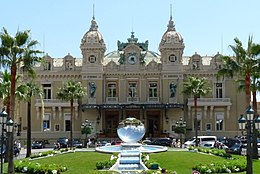
\includegraphics[width=4.5cm]{Monaco_-_panoramio_(138).jpg}}
\vspace*{.5cm}

\dleft{10cm}{
    \begin{enumerate}
        \item Rappeler l'aire d'un disque de rayon 1.
        \item On génère aléatoirement un point $\pc{M}{x}{y}$ dans le carré de côté 1.
    \end{enumerate}
    
    \begin{enumalph}
        \item Quelle est la probabilité que le point $M$ appartienne au quart de disque ?
        \item Exprimer la longueur $OM$ en fonction de $x$ et $y$.
        \item En déduire une inéquation caractérisant les points appartenant au quart de disque.
    \end{enumalph}
}
{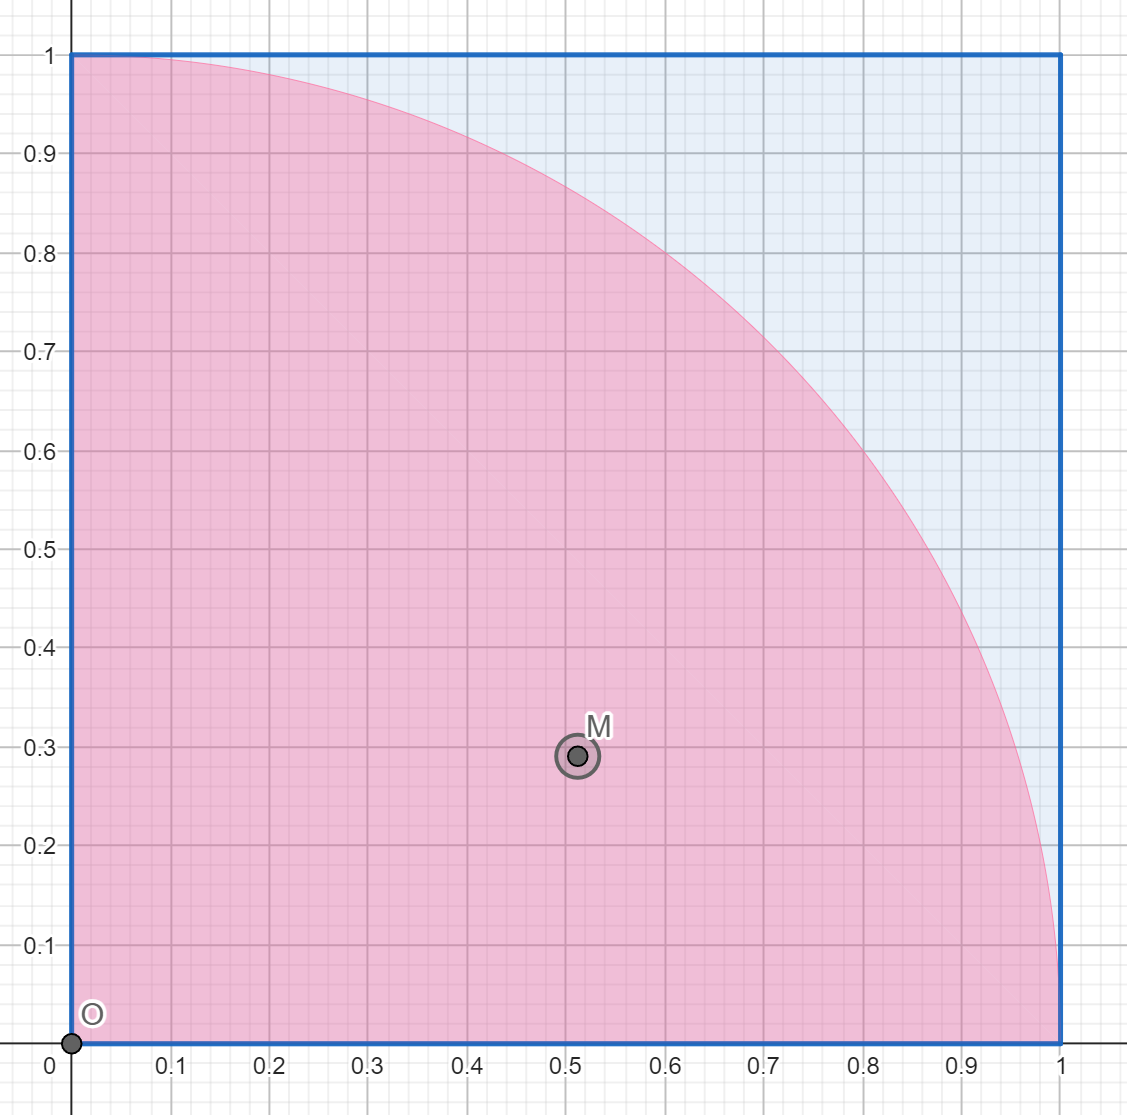
\includegraphics[width=6.5cm]{monte_carlo3.png}}
\begin{enumerate}[label=\textbf{3.}]
    \item  \textbf{Utilisation d'un algoritme :}
\end{enumerate}
\begin{enumalph}
    \item Compléter la deuxième partie de l'activité Capytale \textbf{0812-5226948}. 
    \item Quelle approximation de $\pi$ obtient-on avec 100 points ? 1000 points ? 100 000 points ?
\end{enumalph}
\end{document}